%Chapter 6

\renewcommand{\thechapter}{6}

\chapter{Distributed Octupole Lattice}



%% Following is copy of HB paper

This chapter discusses preliminary testing of a distributed octupole lattice, conducted in parallel with preparations for the more robust single-channel design.

\section{Theory}

The primary focus of this paper is the second consideration, a distributed octupole lattice. Thin nonlinear inserts are distributed at even intervals about the ring ($90^o$ points, see Fig. \ref{N4lattice}).  The alternative lattice uses printed circuit octupoles with the same aspect ratio as the standard UMER PC quad, which are seated in unused quadrupole mounts at the mid-point of the FODO cell. 

The distributed octupole lattice is natively suited to the UMER structure, allowing the installation of octupoles with minimal disruptions to the ring (utilizing existing mounts and power supplies). However, it is a coarse approximation of the quasi-integrable octupole lattice and it is expected that these approximations will limit the extent to which the Hamiltonian $H_N$ is conserved.

A key liberty taken with the quasi-integrable theory is the requirement that $\beta_x=\beta_y$ throughout the nonlinear element. In this case, $\beta_x \approx \beta_y$, with differences on order 15\%. The other approximation is that the PC octupole is fringe-dominated, meaning the longitudinal profile is not flat top and therefore the magnet cannot perfectly meet the requirement that $V_{oct} = 1/\beta^3 =$ constant. Theoretical calculations of the UMER magnets predict that fringe fields cancel due to the relatively short magnet length.\cite{VenturiniThesis} It is yet to be seen if this cancellation will help preserve the nonlinear invariant. Octupole models used in simulations shown here utilize a hard-edged approximation. 

% -- unsure about this section
To meet the $n-\pi$ phase advance requirment from the quasi-integrable theory, the distributed octupole lattice can be tuned to have a tune of $4+\delta 2\pi$, where $\delta$ indicates the phase advance through the octupoles. For a turn length of 11.52 m, effective octupole length of 5.2 cm and tune near 4, the phase advance through the octupoles will be near $\psi = 0.07 *2\pi$. 





\section{Distributed Octupole Lattice Simulations}

\subsection{Various configurations of distributed octupoles}
%todo: other variations? (N:18,12,6,3,2,1 octupoles)



\begin{figure}
\subfigure[N36 octupole lattice]{ \centering
	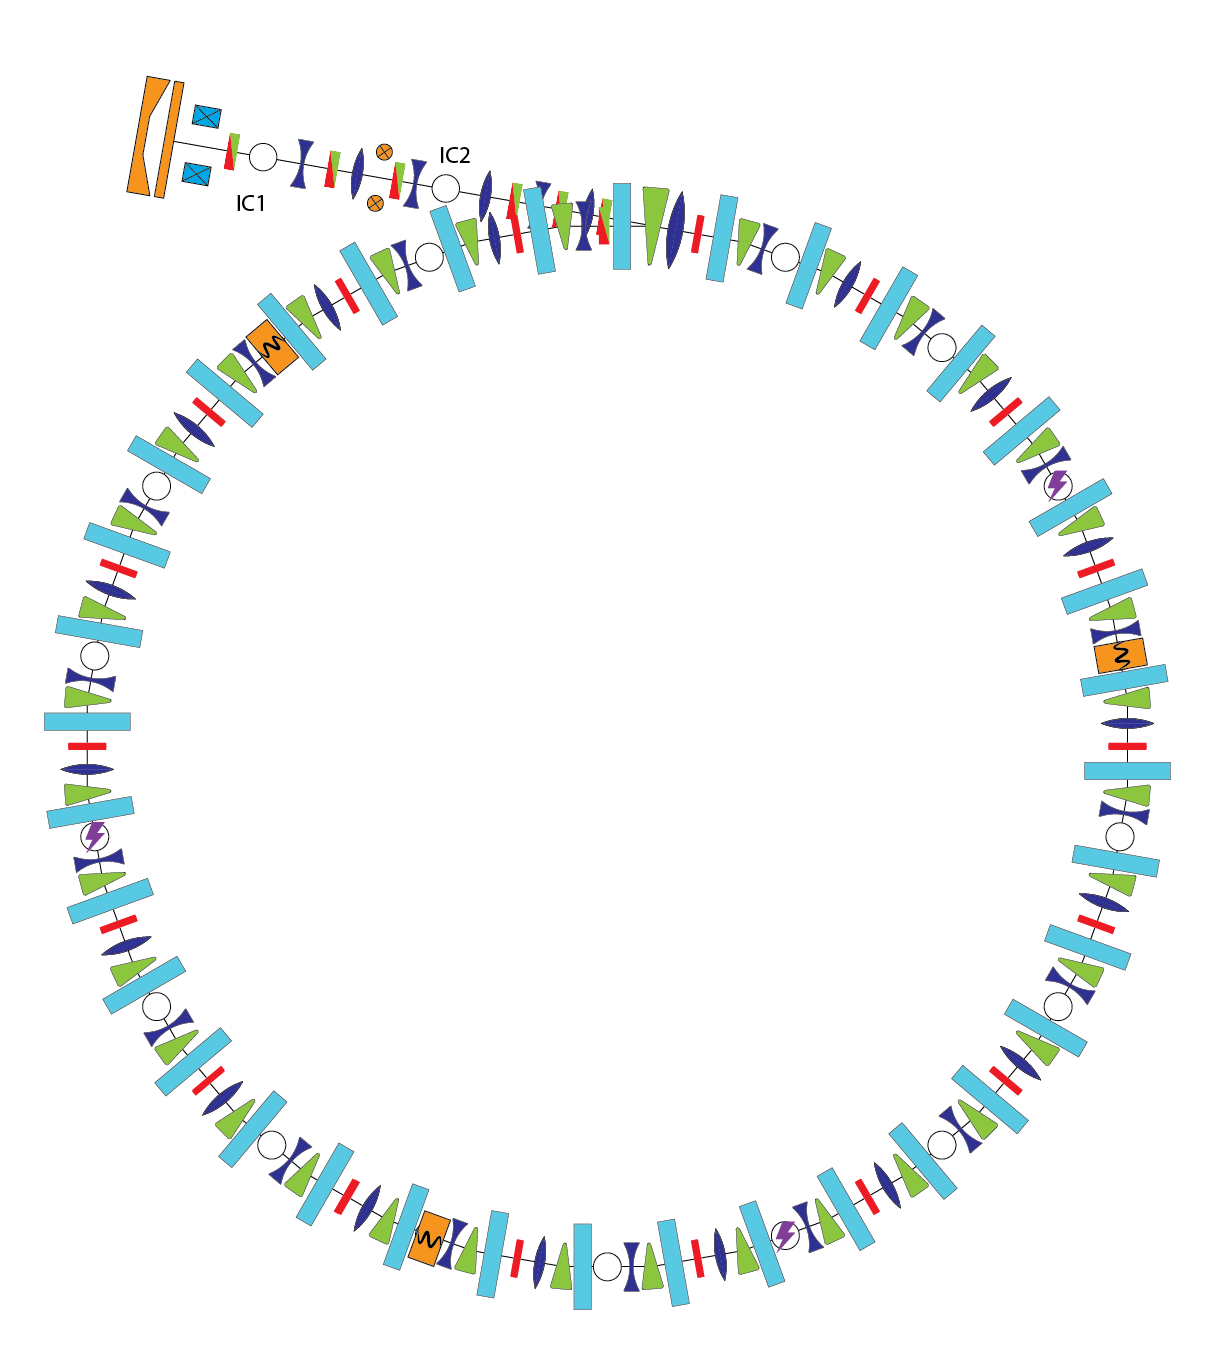
\includegraphics[width=.3\textwidth]{umer-diagram/altlat_N36octu_full_ring.png}
	}
\subfigure[N9 octupole lattice]{ \centering
	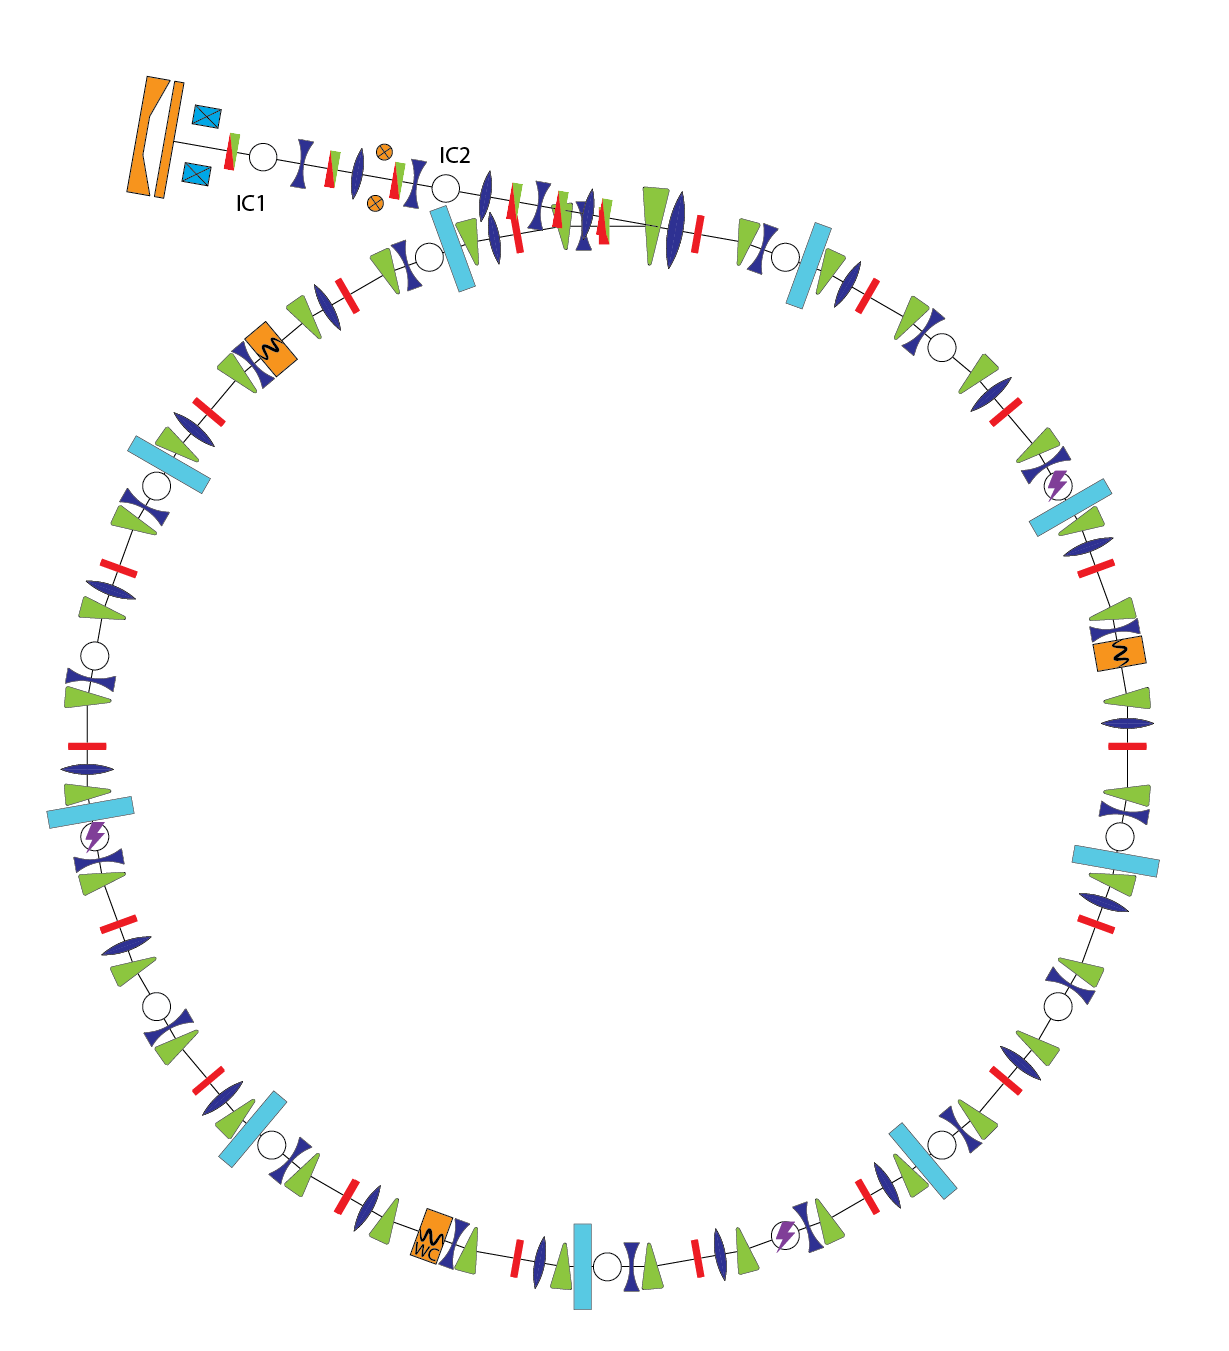
\includegraphics[width=.3\textwidth]{umer-diagram/altlat_N9octu_full_ring.png}
	}
\subfigure[N4 octupole lattice]{ \centering
	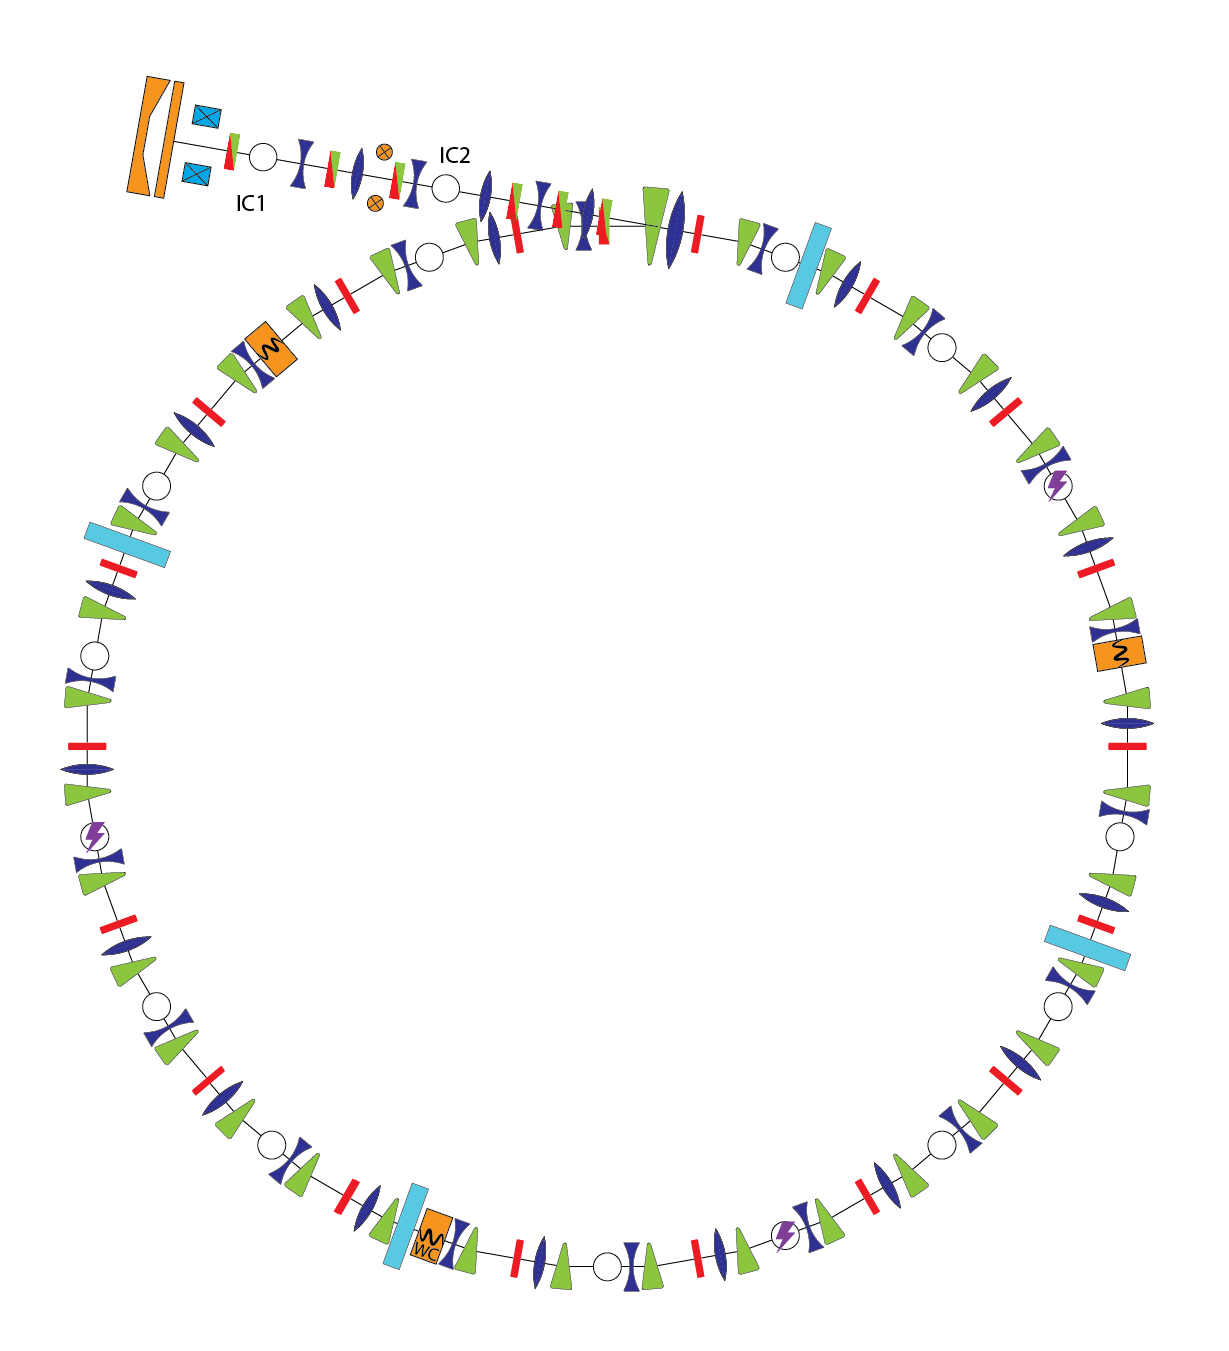
\includegraphics[width=.3\textwidth]{umer-diagram/altlat_N4octu_full_ring.png}
	}	
\caption{A selection of distributed octupole lattices tested for dynamic aperture and tune spread. }
\label{fig:Noctulattices}
\end{figure}

\begin{table}
\centering
	\begin{tabular}{|c|c|c|c|}
	\hline
	\# octupoles & spacing [m] & $\Delta \nu_x$ & $\Delta \nu_y$ \\
	\hline
	36 & 0.32 & 0.11 & 0.11 \\
	9 & 1.28 & 0.45 & 0.46 \\
	4 & 2.88 & 1.01 & 1.03 \\
	\hline
	\end{tabular}
\caption{Configurations considered for distributed octupole lattices. $\Delta \nu$ is tune advance between octupole centers in Elegant simulation.}
\label{tab:Noctlattices}
\end{table}




\subsection{Frequency Map Analysis} 

%todo: add to this section other configurations considered. 

The idea of the distributed octupole lattice was first explored in the Elegant code, which allows beam tracking through third order matrices and symplectic elements.\cite{elegant} Frequency map analysis shows the dynamic aperture is largest for an evenly distributed N4-octupole lattice With an octupole strength of $200 T/m^3$, which corresponds to approximately 2.66 A in the physical octupoles, we see a tune shifts up to $ \Delta \nu \approx 0.07$. This comes at the cost of operating near the integer resonance band. 

The Elegant calculation was run at $\delta \psi_x = 1.06 *2 \pi$, $\delta \psi_y = 1.08 *2 \pi$ between octupoles (ring tune of $\nu_x=4.45$, $\nu_y=4.54$), slightly displaced from the ideal $\delta \psi_x =  \delta \psi_y = 2 \pi$ between octupoles. At this offset, the integer resonance band $\nu_x=\nu_y$ is visible in both configuration and tune space as an evacuated band, as seen in Fig. \ref{fma}. This integer band is destructive and cannot be mitigated by increasing octupole strength to drive up tune spread; The maximum externally induced tune spread is fixed, while the dynamic aperture decreases with octupole current (and amplitude dependent tunes scale accordingly). 

A comparable analysis for single channel design was done in Elegant. The single channel octupole is expected to have a maximum tune shift of roughly twice what is expected in the N4 lattice ($\delta \nu \approx 0.23$), and less apparent sensitivity to the $\nu_x=\nu_y$ band.

\begin{figure}
	\subfigure[]{\centering
    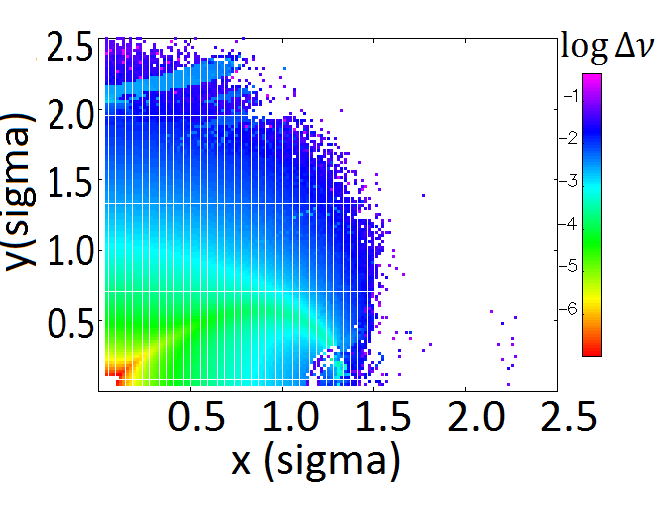
\includegraphics[width=0.5\textwidth]{6.figures/paper_umer_oct_A.png}
	}
	\subfigure[]{\centering
	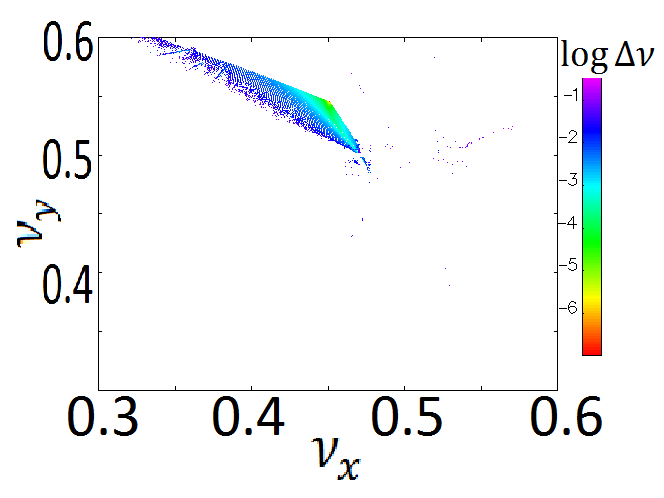
\includegraphics[width=0.5\textwidth]{6.figures/paper_umer_oct_nu.png}
	}
 	\caption{Frequency Map Analysis of N4 lattice in configuration and tune space}
   \label{fig:N4fma}
\end{figure}







\subsubsection{Tracking Hamiltonian Invariant}

Simulations of N4 distributed lattices in the Elegant and Warp codes predict enhanced stability near the ideal tune operating point. 

\begin{figure}[]
   \centering
    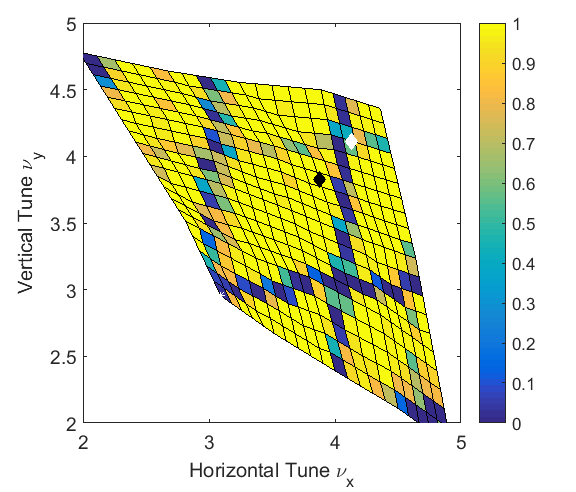
\includegraphics[width=0.5\textwidth]{6.figures/warp_tune_scan_plot.png}
 	\caption{Tune scan, simulated with WARP. Color axis shows particle survival over a range of operating points. Black marker indicates operating point $\nu_x=3.88$, $\nu_y=3.83$, while white marker indicates $\nu_x=4.13$, $\nu_y=4.11$.}
   \label{fig:warpscan}
\end{figure}

In comparison, invariant tracking through the N4 distributed lattice shows much larger amplitude oscillations in $H_N$, most likely due to the approximations on the nonlinear portion of the lattice. For the WARP model, we use hard edged elements in the alternative lattice configuration. Octupoles of length 5.2 cm and peak strength $75 T/m^3/A$ are placed at 2.88 m intervals. 

Two cases are considered:  The historically utilized alternative lattice operating point $I_F=I_D=0.87 A$, which has a tune (as calculated in WARP) of $\nu_x=3.88$, $\nu_y=3.83$ and $I_F=0.938 A$, $I_D=0.944 A$, with tunes $\nu_x=4.13$, $\nu_y=4.11$. The two operating points are marked in Fig. \ref{fig:warpscan}. 

\begin{figure}[]
   \centering
	\subfigure[]{ \centering
    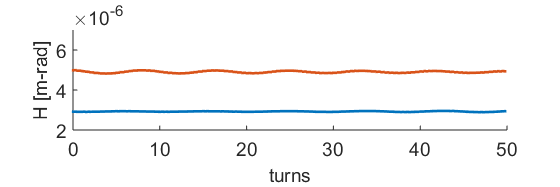
\includegraphics[width=\textwidth]{6.figures/Ioct=0_F0870_D0870.png}
	}
	\subfigure[]{\centering
    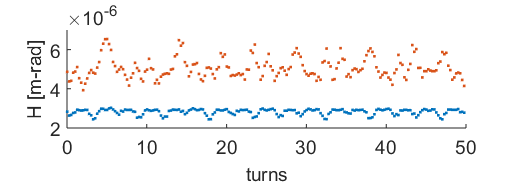
\includegraphics[width=\textwidth]{6.figures/Ioct=2_F0870_D0870.png}
	}
	\subfigure[]{ \centering
    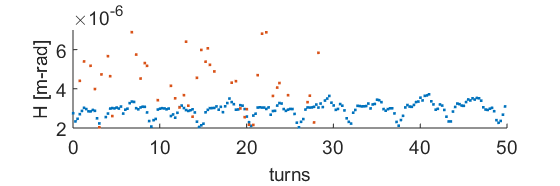
\includegraphics[width=\textwidth]{6.figures/Ioct=4_F0870_D0870.png}
	}
 	\caption{Invariant $H_N$ for N4 distributed lattice at $\nu_x=3.88$, $\nu_y=3.83$}
   \label{fig:N4invar1}
\end{figure}

\begin{figure}[]
	\subfigure[]{ \centering 
    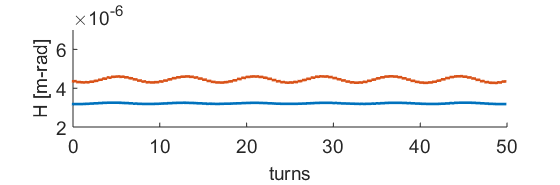
\includegraphics[width=\textwidth]{6.figures/Ioct=0_F09385_D09435.png}
	}
	\subfigure[]{ \centering
    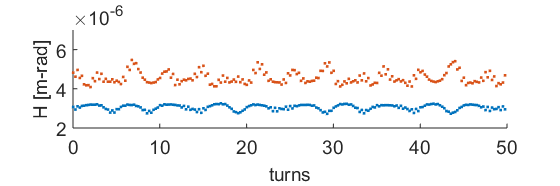
\includegraphics[width=\textwidth]{6.figures/Ioct=2_F09385_D09435.png}
	}
	\subfigure[]{ \centering
    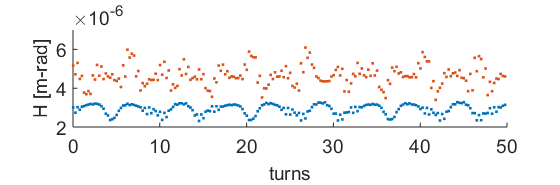
\includegraphics[width=\textwidth]{6.figures/Ioct=4_F09385_D09435.png}
	}
 	\caption{Invariant $H_N$ for N4 distributed lattice at $\nu_x=4.13$, $\nu_y=4.11$}
    \label{fig:N4invar2}
\end{figure}

One expects the invariant to be perfectly conserved in the linear case ($I_{oct}=0$). Also, decrease of dynamic aperture with increasing octupole strength is can be seen through high-amplitude unstable chaotic orbits leaving the system. Recall, for the nonlinear invariant to be conserved, particles must have continuous motion through the octupole elements otherwise chaotic, unbounded orbits are permitted.\cite{Danilov2010} In the case continuous motion (or quasi-continuous, allowing for linear inserts between octupoles) cannot be maintained, we expect the invariant quantity to be less bounded. As seen Fig. \ref{fig:N4invar1} and Fig. \ref{fig: N4invar2}, particles seem to gain stability as the external focusing nears the $\nu_x=\nu_y=4.07$ condition. However, simulations at this operating point yield poor results, and the invariant is not well conserved. 

While the Hamiltonian is not well conserved, long term stability (past the tested 50 turns) may be possible. A natural extension of this work is to include predicted experimental errors into the invariant calculation, as well as extend consideration to a wider range of operating points.






\begin{table}[]
%   \vspace*{-.5\baselineskip}
   \centering
   \caption{Results of invariant tracking in N4 octupole lattice.}
   \begin{tabular}{lccc} \hline
	   $\nu_x=4.13$ & $\nu_y=4.11$\\ \hline
       \textbf{$I_{oct}$ [A]} & \textbf{$\langle H_N \rangle$}        &RMS variation             & \% variation peak-to-peak  \\
           0        & 3.22E-6    &2.3E-8      & 2.4       \\ %[3pt]
          0.5       & 3.17E-6     &4.2E-8     & 6.2       \\ %[3pt]
           2.0        & 3.05E-6    &1.1E-7     &17.6       \\ %[3pt]
           4.0      & 2.91E-6      &2.1E-7   & 33.5        \\ \hline
	   $\nu_x=3.88$ & $\nu_y=3.83$\\ \hline
       \textbf{$I_{oct}$ [A]} & \textbf{$\langle H_N \rangle$}          &RMS variation          & \% variation \\
		& & & peak to peak\\
           0        & 2.92E-6      &1.5E-8    & 2.3       \\ %[3pt]
          0.5       & 2.90E-6      &3.5E-8    & 6.8       \\ %[3pt]
           2.0        & 2.82E-6     & 1.0E-7    & 20.8       \\ %[3pt]
           4.0      & 2.93E-6       & 1.4E-7   & 59.9        \\

   \end{tabular}
   \label{l2ea4-t1}
%   \vspace*{-\baselineskip}
\end{table}


\section{Experimental Setup}


\begin{figure}[]
   \centering
   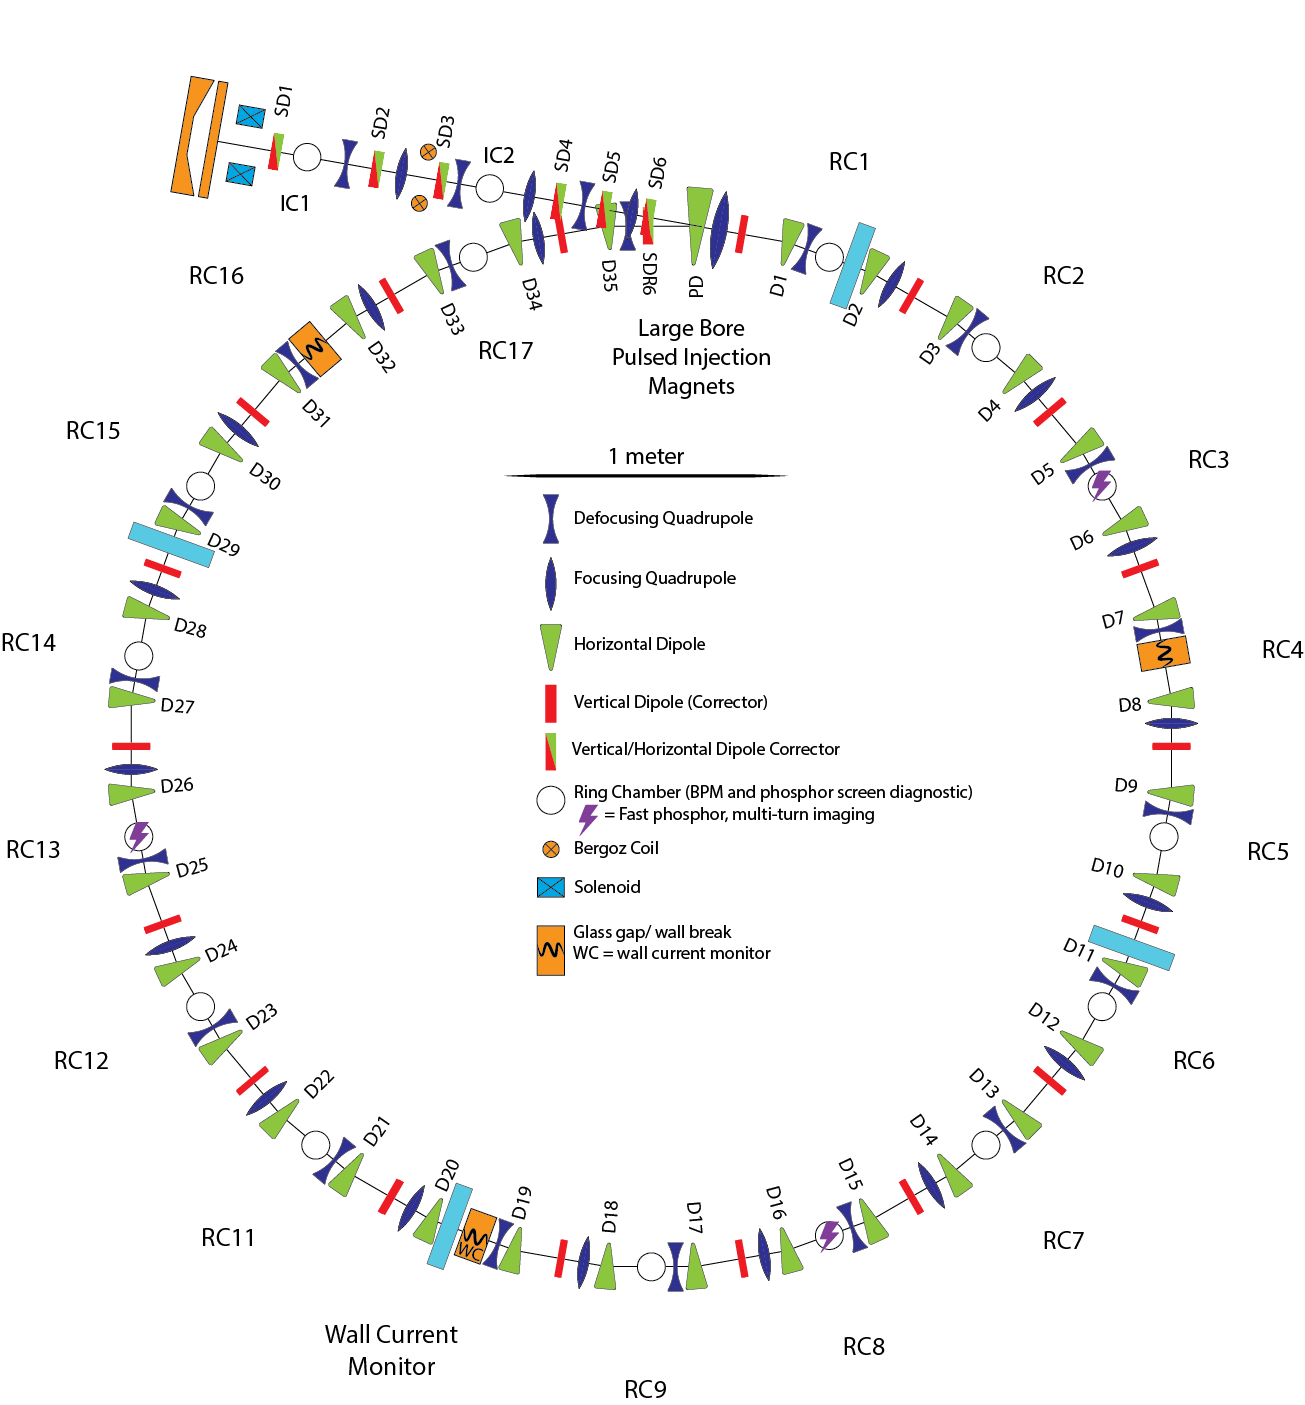
\includegraphics[width=\textwidth]{umer-diagram/altlat_N4octu_full_ring_labels.png}
   \caption{N4 octupole lattice imposed on alternative lattice, large light-blue elements indicate octupole position.}
   \label{fig:N4lattice}
\end{figure}



\section{Preliminary Measurements}

\begin{figure}[]
   \centering
    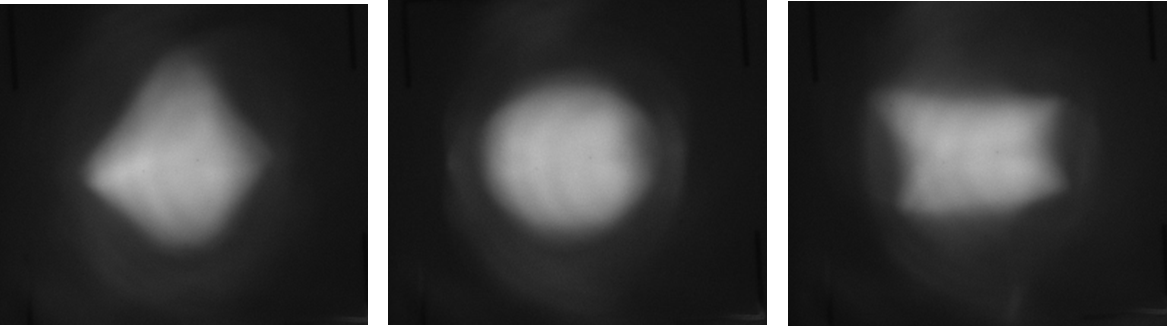
\includegraphics[width=\textwidth]{6.figures/oct_profile.png}
 	\caption{Beam profile after 1 pass through octupole, imaged using phosphor screen. From left to right: $I_{oct} >0$, $I_{oct} =0$, $I_{oct} <0$}
   \label{fig:beam-pass-through-octu}
\end{figure}


\subsection{Tune Scan}

\begin{figure}[]
	\subfigure[Alternative lattice tune scan ]{
	\centering
    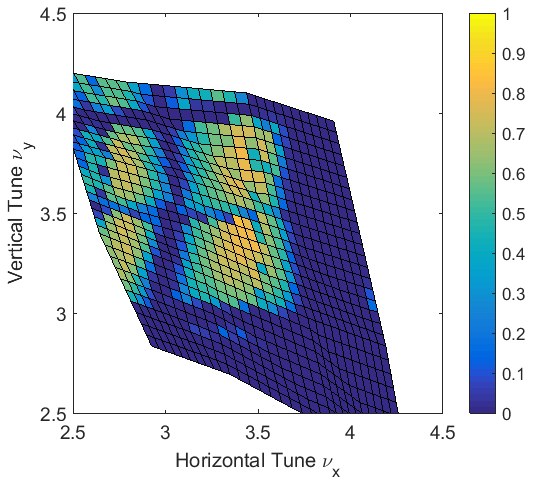
\includegraphics[width=0.48\textwidth]{6.figures/pencil_tune_scan_plot_currentspace_Oct0.png}
	}
	\subfigure[N4 lattice tune scan with octupoles powered at 0.5 A]{
	\centering
    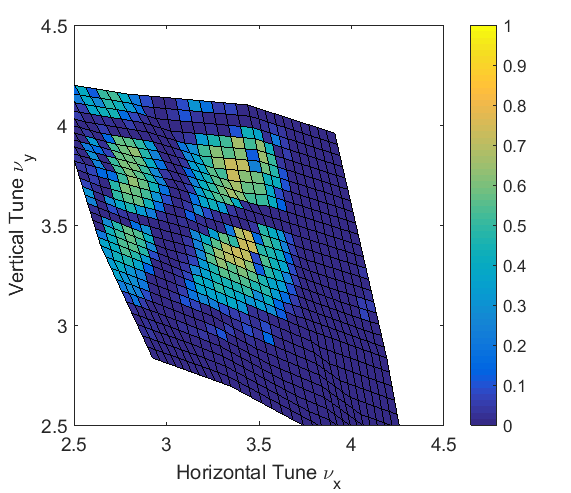
\includegraphics[width=0.5\textwidth]{6.figures/pencil_tune_scan_plot_currentspace_Oct5.png}
	}
 	\caption{Tune scan data for 0.6 mA "pencil" beam, beam survival plot at 25 turns. Color axis is peak beam current normalized to 10th turn.}
   \label{fig:oct-tune-scan-pencil}
\end{figure}


In preparation for N4 lattice testing, measurements are taken on the alternative lattice to gauge beam losses over a variety of operating parameters. The tune scan technique, described in more detail in \cite{tunescan}, measures variations in beam losses as a function of quadrupole strength in two families of quadrupoles (horizontally focusing and defocusing, notated as $I_F$ and $I_D$). Fig. \ref{fig:oct-tune-scan-pencil} shows beam survival measurements of the 0.6 mA beam for a range of quadrupole values.  Transformation to tune-space was done using WARP simulations with hard-edged elements and a thin-lens model of dipole edge focusing. The obvious integer resonance bands are used to orient the measurement in tune-space. An offset of $\nu_x = -0.45$ and $\nu_y = -0.35$ from the WARP prediction is necessary to line up integer bands. 

The tunescan shows broad bands at the even integer tune resonances. As this N4 lattice is intended to be run at $\nu_x=\nu_y=4 + \delta$, tuning the beam closer to this operating point will be necessary if any beneficial effect is to be observed over the integer band losses. With octupoles on (Figs. \ref{fig:oct-tune-scan-pencil},\ref{fig:beam-pass-through-octu}), no apparent increase in dynamic aperture is seen. 



\subsubsection{Errors: Beam Matching and Steering}

The beam matching quadrupoles and steering correctors were optimized to a single operating point, at $I_F=I_D = 0.87$ A. It is expected that the accrued errors in the match and the steering grow with greater distance from the ideal operating point, although it is not clear that they accrue anisoptropically.
%Steering in UMER is significantly complicated by the presence of a nominally 400 mG vertical Earth field component, which provides approximately 20 degrees of bending over a 32 cm FODO cell. The horizontal component, with maximum value approximately 200 mG, also contributes to the dynamics. The ideal closed orbit therefore is not centered on the beam pipe, but rather arcs across a FODO cell through the centers of the quadrupoles, complicating the steering procedure. 

The steering solution for this operating point had first turn horizontal offsets in the quadrupoles  of RMS 0.5 mm with a maximum of 1.3 mm. Vertically, RMS offsets are 3.2 mm with maximum value of approximately 8.5 +- 0.5 mm. The contribution of these steering errors can be seen in the width of the integer resonance bands in the tune scan data (Fig. \ref{data}). More precise control of the steering will likely improve this characteristic by reducing the steering error for all operating points.

The beam match was not well-tuned, with percent RMS variations of 33\% in the horizontal and 28\% in the vertical. More accurate matching solutions have been demonstrated in UMER, up to standard deviations of 0.17 mm horizontally and 014 mm vertically for the 6 mA beam. \cite{HaoThesis}


\section{Conclusion}

In conclusion, UMER is equipped to test quasi-integrable octupole lattices. Insight has been built into the behavior of the N4 octupole lattice, which has potential to be a testbed for quasi-integrable dynamics. However, the proximity to an integer resonance band may ultimately limit its usefulness and implementation, at least with short octupole elements. On UMER, the large $\nu_x = 4$ band overshadows any resonant loss mitigation induced by the octupoles. 


